\documentclass[10pt]{article}

\usepackage[utf8]{inputenc}
\usepackage[T1]{fontenc}
\usepackage[english]{babel}

\usepackage{url}
\usepackage{xcolor}
\usepackage[version=3]{mhchem}
\usepackage[top=2cm,bottom=2cm,left=2cm,right=2cm]{geometry}

\usepackage{tikz}
\usetikzlibrary{shadows}

\usepackage{palatino}
\setlength{\parskip}{1.5ex plus 0.5ex minus 0.5ex}
\setlength{\parindent}{0em}
\usepackage{setspace}
\AtBeginDocument{\onehalfspacing}

\usepackage[toc]{multitoc}
\setlength{\columnsep}{2cm}
\renewcommand{\columnseprule}{.14pt}

% ------------------------------------------------------------------------------
% section format
% ------------------------------------------------------------------------------
\usepackage{titlesec}
\titleformat*{\section}{\sffamily\Large\bfseries}
\titleformat*{\subsection}{\sffamily\large\bfseries}
\titleformat*{\subsubsection}{\sffamily\bfseries}

% ------------------------------------------------------------------------------
% listing package
% ------------------------------------------------------------------------------
\usepackage{listings}
\definecolor{keycolor}{RGB}{172, 42, 42}

\lstset{% general command to set parameter(s)
language=[LaTeX]TeX,
numbers=left,
numberstyle=\tiny\color{black!50},
identifierstyle=,
basicstyle={\small\color{black!95}\ttfamily},
stringstyle=,
keywordstyle=\bfseries\color{keycolor},
commentstyle=\color{black!50},
backgroundcolor=,
emph={ifthenelse,equal,draw,node,tikzstyle,pgfsetlayers,pgfkeys,ProvidesPackage,
     colorlet,default,store, in, cd, setOrbitalDrawing, orbitalDrawing,
     path,text,RequirePackage,pgfdeclarelayer,usetikzlibrary,command},
emphstyle=\bfseries\color{red!60!black},
emph=[2]{orbital,drawLevel,@alobe},
emphstyle=[2]\itshape\color{blue!50!black},
moredelim=[s][\color{green!40!black}]{[}{]},
}

% ------------------------------------------------------------------------------
% new float example
% ------------------------------------------------------------------------------
\usepackage{float}
\newfloat{example}{htbp}{exple}[section]
\floatname{example}{Example}

% ------------------------------------------------------------------------------
% newcommand
% ------------------------------------------------------------------------------
\usepackage{xspace}
\newcommand*{\cmd}[1]{{\ttfamily\color{blue!50!black}$\setminus$#1}\xspace}
\newcommand*{\opt}[1]{{\ttfamily\itshape\color{green!60!black}[<#1>]}\xspace}
\newcommand*{\marg}[1]{{\ttfamily\itshape\color{red!95!black}<#1>}\xspace}
\newcommand{\package}{\textsc{\sffamily\color{blue!50!black}tikzorbiltal}\xspace}

% ------------------------------------------------------------------------------
% hyperref
% ------------------------------------------------------------------------------
\usepackage{hyperref}
\hypersetup{% Modifiez la valeur des champs suivants
pdftex,%               Sets up hyperref for use with the pdftex program
colorlinks=true,%      active les liens
pdfborder={0 0 0},%    bordure des liens
urlcolor=blue!50!black,
linkcolor=,%  Color for normal internal links.
pdfstartpage=1,%       page affichee a l'ouverture du pdf
pdfauthor={Germain Vallverdu},%
pdftitle={tikzorbital package},% 
pdfkeywords={latex,orbital,package,tikz},%
pdfcreator={PDFLaTeX},%
pdfproducer={PDFLaTeX},%
}

% ------------------------------------------------------------------------------
\title{\package Package}
\author{Germain \textsc{Salvato-Vallverdu} \\ \url{<germain.vallverdu@univ-pau.fr>}\\\url{http://gvallver.perso.univ-pau.fr/}}
\date{\today}

\usepackage{tikzorbital}

% ------------------------------------------------------------------------------
\begin{document}
% ------------------------------------------------------------------------------

\maketitle

\begin{abstract}
    This package provides several \LaTeX{} macros in order to draw easily molecular diagrams and atomic orbital of type $s$, $p$ and $d$ inside tikzpicture environment. This documentation gives the syntax of the commands and complete examples of their utilization. The source code is give at the end.
\end{abstract}

{\singlespacing
\tableofcontents
}

\section{Requirements and licence}

\package underlies the \LaTeX{} project public license (lppl) version 1.3 or later (\url{http://www.latex-project.org/lppl.txt}). It requires the following packages which all are usually included in standard texlive or MikTex distribution :

\begin{itemize}
    \item tikz, pgfkeys (part of tikz) and tikz library shapes
    \item ifthen
\end{itemize}

Feel, free to send comments, contribution or suggestion by email.

\section{Installation and utilization}

Download the tarball which contains the files \verb!tikzorbital.sty! and \verb!tikzorbital.pdf! which are respectively the package file and its documentation (\url{http://gvallver.perso.univ-pau.fr/}). After extracting the files, copy them to directories where \LaTeX{} will be able to find them. For example, under Linux operating systems :

\begin{lstlisting}
% for the .sty file
/home/you/texmf/tex/latex/tikzorbital

% for the pdf documentation file
/home/you/texmf/doc/latex/tikzorbital
\end{lstlisting}

Under a macOS operating system the \verb!texmf! directory is not in your home directory but in the \verb!Library! directory.

Package \package do not have any options. After you have copied it in a directory where \LaTeX{} will find it, simply load it as other \LaTeX{} package :

\begin{lstlisting}
\usepackage{tikzorbital}
\end{lstlisting}

All macros provided by \package must be uses inside a tikzpicture environment. The \opt{pos} option of the macro is a position which can be given in the tikz syntax.

Options of macros provided by \package must be given in a \texttt{key = value} syntax. For example :
%
\begin{lstlisting}
\command[option 1 = <value1>, option2 = <value2> ...]{argument}
\end{lstlisting}

\section{Molecular orbital diagrams}

The package \package provides the following command in order to draw easily molecular orbital diagrams :

\cmd{drawLevel}\opt{options}\texttt{\{}\marg{name}\texttt{\}}

This command draw a thick line with zero, one or two electrons which represent the occupation of the orbital and are drew as vertical arrows which indicate the spin of each electron. \marg{name} is the name of the orbital and is used in order to define anchors which could be used in order to draw correlation lines or to add labels (see example \ref{expl:molecular_diagram}). The following anchor are created :

\begin{itemize}
    \item \texttt{left name} : at the left of the orbital level
    \item \texttt{right name} : at the right of the orbital level
    \item \texttt{middle name} : at the middle of the orbital level
\end{itemize}

The following \opt{options} are available :
%
\begin{description}
    \item \opt{elec} : Number of electrons, \texttt{<value>} must be one of \{\texttt{up, down, updown, pair}\} where \texttt{pair} and \texttt{updown} have got the same effect.\\
    \texttt{default = no}
    
    \item \opt{pos} : left position of the level\\
    \texttt{default  = \{(0,0)\}}
    
    \item \opt{width} : level width\\
    \texttt{default = 2}    
    
    \item \opt{style} : a set of tikz commands which define the way levels have to be drawn\\
    \texttt{default = \{line width = 2pt, color = black!80, line cap = round\}}
    
    \item \opt{spinstyle} : a set of tikz commands which define the way the arrows which represents the electrons have to be drawn\\
    \texttt{default = \{very thick, color = red!80, -stealth\}}
    
    \item \opt{spinlength} : length of spin arrows \\
    \texttt{default = 1}
\end{description}

Note that if the value of an option contains comma or parenthesis, you should enclose its in curly brace.

Example \ref{expl:molecular_diagram} shows how to use \cmd{drawLevel} for molecule \ce{HHe}.

\begin{example}[h]
\begin{minipage}{0.6\textwidth}
\begin{lstlisting}
\begin{tikzpicture}
   \drawLevel[elec = up, pos = {(0,0)}, width = 2]{1sH}
   \drawLevel[elec = updown, pos = {(6,-2)}, width = 2]{1sHe}

   \drawLevel[elec = pair, pos = {(3,-3)}, width = 2]{sigma}
   \drawLevel[elec = up, pos = {(3,3)}, width = 2]{sigmastar}

   \draw[dashed] (right 1sH) -- (left sigma)
         (right 1sH) -- (left sigmastar)
         (left 1sHe) -- (right sigmastar)
         (left 1sHe) -- (right sigma) ;

   \node[left] at (left 1sH) {\ce{1s_H}} ;
   \node[right] at (right 1sHe) {\ce{1s_{He}}} ;
   \node[left] at (left sigma) {$\sigma$};
   \node[left] at (left sigmastar) {$\sigma^*$};
\end{tikzpicture}
\end{lstlisting}
\end{minipage}
\hfill
\begin{minipage}{0.39\textwidth}
\centering
\begin{tikzpicture}[scale=0.7]
     \drawLevel[elec = up, pos = {(0,0)}, width = 2]{1sH}
     \drawLevel[elec = updown, pos = {(6,-2)}, width = 2]{1sHe}

     \drawLevel[elec = pair, pos = {(3,-3)}, width = 2]{sigma}
     \drawLevel[elec = up, pos = {(3,3)}, width = 2]{sigmastar}

     \draw[dashed] (right 1sH) -- (left sigma)
           (right 1sH) -- (left sigmastar)
           (left 1sHe) -- (right sigmastar)
           (left 1sHe) -- (right sigma) ;

     \node[left] at (left 1sH) {\ce{1s_H}} ;
     \node[right] at (right 1sHe) {\ce{1s_{He}}} ;
     \node[left] at (left sigma) {$\sigma$};
     \node[left] at (left sigmastar) {$\sigma^*$};
\end{tikzpicture}
\end{minipage}
\caption{Example of the molecular diagram of the molecule \ce{HHe+} drew with the command \cmd{drawLevel}.}
\label{expl:molecular_diagram}
\end{example}

\section{Molecular orbitals drawings}

The package \package, provides the command \cmd{orbital} in order to draw atomic orbital $s$, $p$ or $d$. The general syntax is :

\cmd{orbital}\opt{options}\{\marg{type}\}

where \marg{type} is the type of the atomic orbital : \texttt{lobe, s, px, py, pz, dxy, dxz, dyz, dx2y2} or \texttt{dz2}. See example \ref{expl:all_OA} to see all atomic orbital types. The \texttt{lobe} type simply draw one lobe of a $p$ or $d$ atomic orbital and may be used, for example, to draw hybrid orbital. With the \texttt{lobe} type you can also represent electrons as small spheres inside the orbital.

\begin{minipage}{.75\textwidth}
\begin{lstlisting}
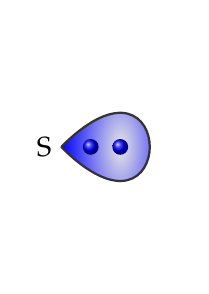
\begin{tikzpicture}
    \node (s) {S};
    \orbital[nelec = 2, scale = 1.5, pos = (s.east)]{lobe}
\end{tikzpicture}
\end{lstlisting}
\end{minipage}
\begin{minipage}{.25\textwidth}
\centering
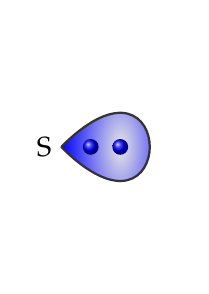
\begin{tikzpicture}
    \node (s) {S};
    \orbital[nelec = 2, scale = 1.5, pos = (s.east)]{lobe}
\end{tikzpicture}
\end{minipage}

\subsection*{General options}

The following options, allow to change the position, the aspect and the size the atomic orbital. They are available for all type of atomic orbital.  :
%
\begin{description}
    \item \opt{pos} : position of the center of the atomic orbital\\ 
    \texttt{default = \{(0,0)\}}
        
    \item \opt{scale} : scaling factor\\
    \texttt{default = 1}
    
    \item \opt{opacity} : opacity of the atomic orbital. Useful if you wish to superimpose atomic orbital\\
    \texttt{default = 1}
\end{description}

\subsubsection*{Color options}

The color of atomic orbitals can be selected with options : \opt{pcolor}, \opt{ncolor} or \opt{color}. The options \opt{pcolor} and \opt{ncolor} stand for the positive and the negative lobes of $p$ or $d$-type atomic orbitals. The \opt{color} option define the color of $s$-type or \texttt{lobe}-type orbital. For these types of atomic orbital, if no color is given the \opt{pcolor} is used.

\begin{description}
    \item \opt{color} : color of the atomic orbital for $s$-type or \texttt{lobe}-type orbital \\
    \texttt{\opt{pcolor} is used}
    
    \item \opt{pcolor} : color of the positive lobe (or color for $s$ and $lobe$-type orbital if \opt{color} is not given)\\
    \texttt{default = blue}
    
    \item \opt{ncolor} : color of the negative lobe (for $p$ and $d$-type orbital only)\\
    \texttt{default = black!30}
\end{description}

\subsubsection*{\texttt{lobe}-type specific options}

The following options will have an effect only for the \texttt{lobe} type :

\begin{description}   
    \item \opt{rotate} : rotation of the atomic orbital\\
    \texttt{default = 0}
    
    \item \opt{nelec} : number of electron to draw inside the lobe\\
    \texttt{default = 0}
\end{description}

\subsubsection*{examples}

Example \ref{expl:all_OA} shows all atomic orbital types available. In order to decide the type of the atomic orbital you need, look at the axes definition below :

\begin{center}
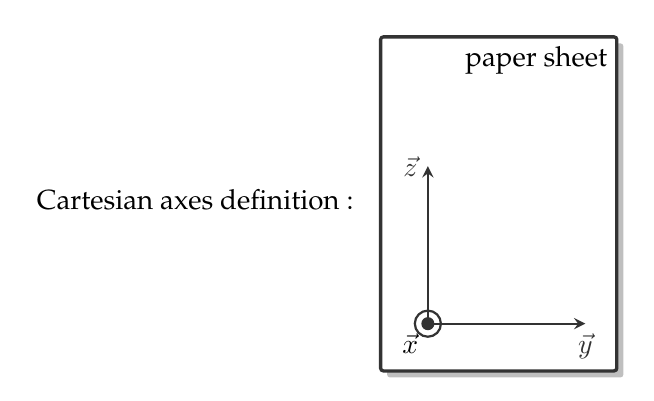
\begin{tikzpicture}[scale = 2]
    \tikzstyle{axe} = [-stealth, thick, color = black!80]
    \draw[very thick, draw = black!80, fill = white, rounded corners = 1pt, drop shadow] (-.3,-.3) rectangle (1.2,1.821) node (corner) {};
    \node[below left] at (corner) {paper sheet};
    \draw[axe] (0,0) -- (1,0) node[below] {$\vec{y}$};
    \draw[axe] (0,0) -- (0,1) node[left] {$\vec{z}$};
    \node[circle, fill = black!80, scale = .5] at (0,0) {};
    \node[circle, draw, color = black!80, thick, scale = 1] {};
    \node[below left] {$\vec{x}$};
    \node[left, xshift = -2mm] at (current bounding box.west) {Cartesian axes definition :};
\end{tikzpicture}
\end{center}

\begin{example}[htbp]
\begin{minipage}{.49\textwidth}
\begin{lstlisting}
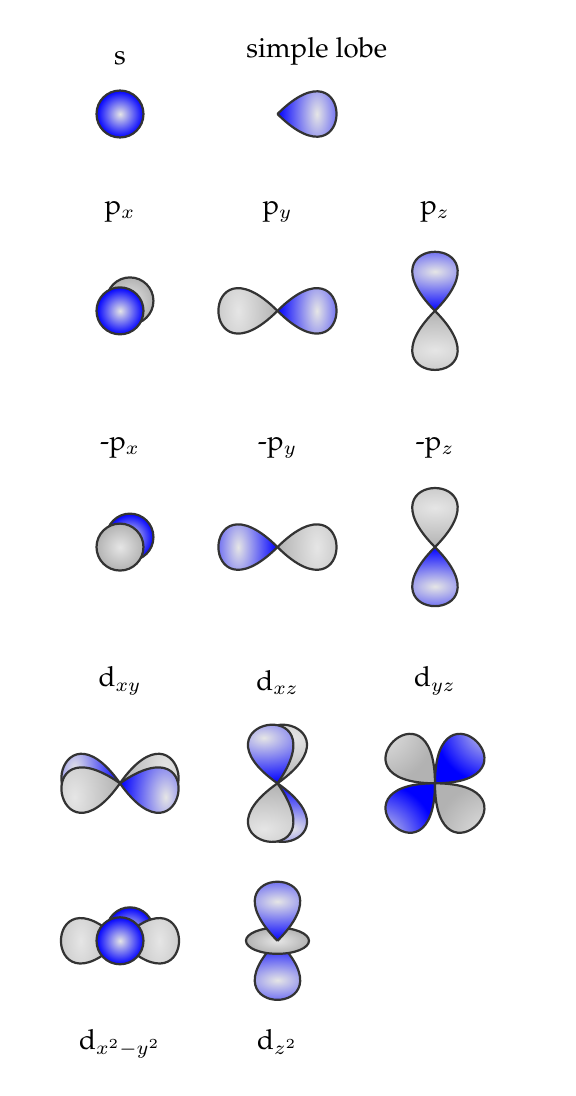
\begin{tikzpicture}
    \orbital[pos = {(2,5.5)}]{lobe}
    \node[above] at (2.5,6) {simple lobe};

    \orbital[pos = {(0,5.5)}]{s}
    \node[above] at (0,6) {s};

    \orbital[pos = {(0,3)}]{px}
    \node[above] at (0,4) {p$_x$};
    \orbital[pos = {(2,3)}]{py}
    \node[above] at (2,4) {p$_y$};
    \orbital[pos = {(4,3)}]{pz}
    \node[above] at (4,4) {p$_z$};

    \orbital[pos = {(0,0)}]{-px}
    \node[above] at (0,1) {-p$_x$};
    \orbital[pos = {(2,0)}]{-py}
    \node[above] at (2,1) {-p$_y$};
    \orbital[pos = {(4,0)}]{-pz}
    \node[above] at (4,1) {-p$_z$};    

    \orbital[pos = {(0,-3)}]{dxy}
    \node[above] at (0,-2) {d$_{xy}$};
    \orbital[pos = {(2,-3)}]{dxz}
    \node[above] at (2,-2) {d$_{xz}$};
    \orbital[pos = {(4,-3)}]{dyz}
    \node[above] at (4,-2) {d$_{yz}$};

    \orbital[pos = {(0,-5)}]{dx2y2}
    \node[below] at (0,-6) {d$_{x^2-y^2}$};
    \orbital[pos = {(2,-5)}]{dz2}
    \node[below] at (2,-6) {d$_{z^2}$};
\end{tikzpicture}
\end{lstlisting}
\end{minipage}
\begin{minipage}{.49\textwidth}
\centering
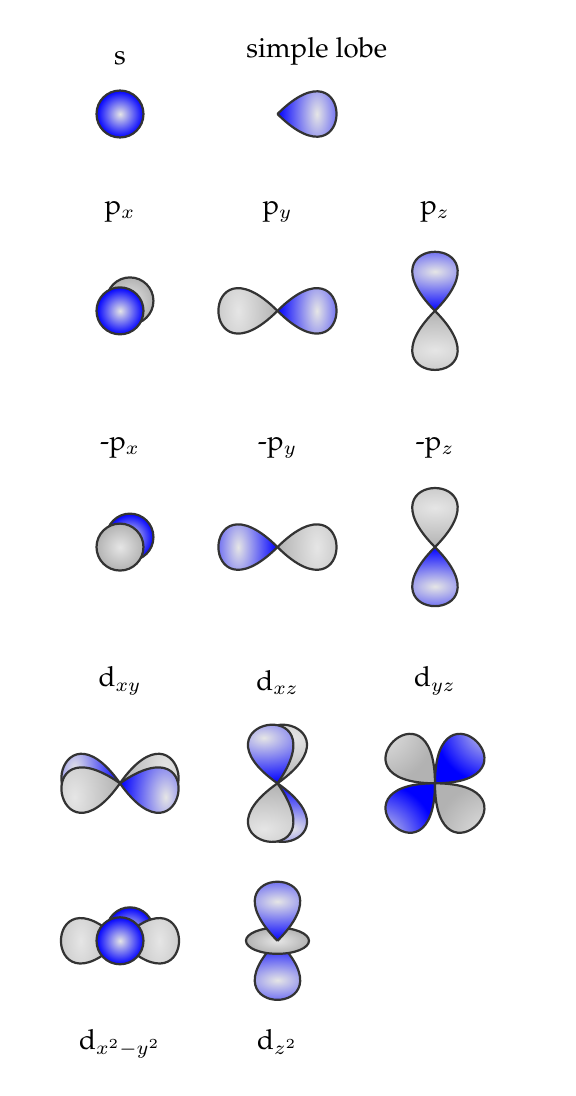
\begin{tikzpicture}
    \orbital[pos = {(2,5.5)}]{lobe}
    \node[above] at (2.5,6) {simple lobe};

    \orbital[pos = {(0,5.5)}]{s}
    \node[above] at (0,6) {s};

    \orbital[pos = {(0,3)}]{px}
    \node[above] at (0,4) {p$_x$};
    \orbital[pos = {(2,3)}]{py}
    \node[above] at (2,4) {p$_y$};
    \orbital[pos = {(4,3)}]{pz}
    \node[above] at (4,4) {p$_z$};

    \orbital[pos = {(0,0)}]{-px}
    \node[above] at (0,1) {-p$_x$};
    \orbital[pos = {(2,0)}]{-py}
    \node[above] at (2,1) {-p$_y$};
    \orbital[pos = {(4,0)}]{-pz}
    \node[above] at (4,1) {-p$_z$};    

    \orbital[pos = {(0,-3)}]{dxy}
    \node[above] at (0,-2) {d$_{xy}$};
    \orbital[pos = {(2,-3)}]{dxz}
    \node[above] at (2,-2) {d$_{xz}$};
    \orbital[pos = {(4,-3)}]{dyz}
    \node[above] at (4,-2) {d$_{yz}$};

    \orbital[pos = {(0,-5)}]{dx2y2}
    \node[below] at (0,-6) {d$_{x^2-y^2}$};
    \orbital[pos = {(2,-5)}]{dz2}
    \node[below] at (2,-6) {d$_{z^2}$};
\end{tikzpicture}
\end{minipage}
\caption{All the atomic orbitals available from the command \cmd{orbital}.}
\label{expl:all_OA}
\end{example}

\clearpage
\section{Atom and hybrid orbitals}

The package \package provides the command \cmd{satom} in order to quickly draw an atom with several orbital lobes around it. The general syntax of the command is :

\cmd{satom}\opt{options}\{\marg{lobes}\}

The \marg{lobes} argument is a comma separated list of lobe definition with the syntax 

\texttt{color/rotation-angle/anchor/number of electrons/scale}

For each element of the list, the command \cmd{satom} draw a lobe at the given
anchor, with the given color, rotation, number of electrons and applies the
scaling factor.

The following options are available in order to customize the drawing :

\begin{description}
    \item \opt{pos} : position of the atom.\\
    \texttt{default = \{(0,0)\}}
    
    \item \opt{name} : name of the atom. Give also the name to the node where the atom is drawn.\\
    \texttt{default = X}
    
    \item \opt{color} : color of the atom.\\
    \texttt{default = green}
    
    \item \opt{opacity} : opacity of the lobe drawn around the atom.\\
    \texttt{default = 0.8}
    
    \item \opt{scale} : A global scaling factor of the whole atom and lobes.\\
    \texttt{default = 1.}
\end{description}

For backward compatibility the \cmd{atom} command is still available. It works
in the same way but without the possibility of applying a scaling factor
individually on each lobe.

Example \ref{exple:atom} show several applications of the command \cmd{satom}.

\begin{example}[htbp]
\begin{minipage}{.78\textwidth}
\begin{lstlisting}
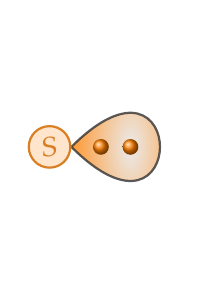
\begin{tikzpicture}
    \satom[color=orange, name=S]{orange/0/east/2/1.}
\end{tikzpicture}
\end{lstlisting}

\begin{lstlisting}
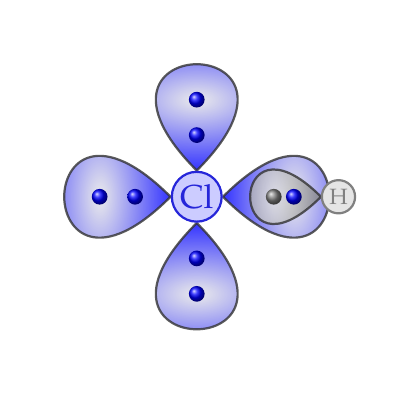
\begin{tikzpicture}
    \atom[name=Cl, color=blue, scale=1.2]{
        blue/90/north/2,
        blue/0/east/1,
        blue/270/south/2,
        blue/180/west/2} 
    \atom[name=H, color=gray, pos={(1.8,0)}, scale=.8]{gray/180/west/1} 
\end{tikzpicture} 
\end{lstlisting}

\begin{lstlisting}
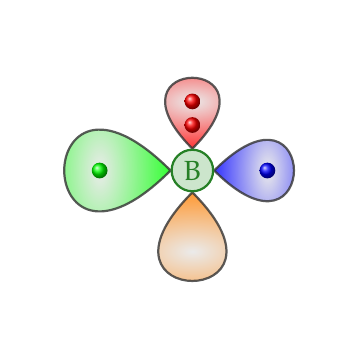
\begin{tikzpicture} 
    \satom[name=B, color=green!50!black]{
        red/90/north/2/.8,
        blue/0/east/1/.9,
        orange/270/south/0/1,
        green/180/west/1/1.2} 
\end{tikzpicture} 
\end{lstlisting}
\end{minipage}
\begin{minipage}{.21\textwidth}
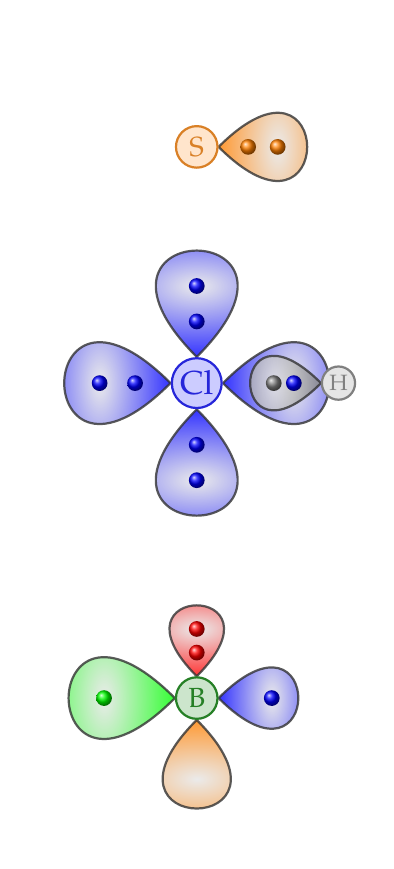
\begin{tikzpicture}
    \satom[color=orange, name=S]{orange/0/east/2/1.}
    
    \atom[name=Cl, color=blue, pos={(0,-3)}, scale=1.2]{
        blue/90/north/2,
        blue/0/east/1,
        blue/270/south/2,
        blue/180/west/2} 
    \atom[name=H, color=gray, pos={(1.8,-3)}, scale=.8]{gray/180/west/1} 
    
    \satom[name=B, color=green!50!black, pos={(0,-7)}]{
        red/90/north/2/.8,
        blue/0/east/1/0.9,
        orange/270/south/0/1,
        green/180/west/1/1.2}
\end{tikzpicture}
\end{minipage}
\caption{Utilization example of the \cmd{satom} command.}
\label{exple:atom}
\end{example}

\clearpage
\section{More customization}

\subsubsection*{Orbital borders and inner color}

It is possible to change the inner color of orbital and the color of orbital borders. These two colors are defined as follow in \package package :

\begin{lstlisting}
% inner color for orbital filling
\colorlet{innerColor}{black!10}
% color for orbital drawing
\colorlet{drawColor}{black!80}
\end{lstlisting}

Thus if you change the definition of these colors you will change the desired color on the drawing of the atomic orbitals.

\subsubsection*{Orbital customization}

You can give a set of tikz options to the command \cmd{setOrbitalDrawing}. This command acts as a tikz style which is applied every time an atomic orbital is drawn. All options give in this command will overwrite default style of atomic orbital. For example, if you want to draw atomic orbital in red with very thick line thickness :

\begin{lstlisting}
\setOrbitalDrawing{{very thick, color = red}}
\end{lstlisting}

\subsubsection*{Change default value globally with pgfkeys}

If you want to change the default value of the \opt{width} option of the \cmd{drawLevel} command or whatever other option for a whole tikzpicture, you can do this using the \lstinline!\pgfkeys! command. You simply have to give to this command one or several options you want to set globally.

All options of a \package's command follow the tree : \texttt{/tikzorbital/command/option}. For example, if you want to change the \opt{width} option of the \cmd{drawLevel} command, you have to write :
%
\begin{lstlisting}
\pgfkeys{tikzorbital/drawLevel/width = 1}
% or
\pgfkeys{tikzorbital/drawLevel/.cd, width = 1}
\end{lstlisting}

\section{Inner macro \cmd{@alobe}}

In order to draw atomic orbital, \package use the inner macro \cmd{@alobe}.

\cmd{@alobe}\{\marg{pos}\}\{\marg{rotation}\}\{\marg{scale}\}\{\marg{color}\}\{\marg{nelec}\}\{\marg{opacity}\}

\cmd{@alobe} macro draw one lobe of $p$ or $d$ orbital and corresponds to the \texttt{lobe} type of \cmd{orbital} (see above). \cmd{@alobe} accepts six arguments :

\begin{enumerate}
     \item[\#1] the position
     \item[\#2] angle of rotation
     \item[\#3] scaling factor
     \item[\#4] the color
     \item[\#5] the number of electron, namely 0, 1 or 2
     \item[\#6] the opacity of the lobe
\end{enumerate}
%
no default are given. For example, the $d_{yz}$ atomic orbital is defined as follow

\begin{lstlisting}
\@alobe{\orbital@pos}{45}{\orbital@scale}{\orbital@pcolor}{0}{\orbital@opacity}   
\@alobe{\orbital@pos}{135}{\orbital@scale}{\orbital@ncolor}{0}{\orbital@opacity} 
\@alobe{\orbital@pos}{225}{\orbital@scale}{\orbital@pcolor}{0}{\orbital@opacity} 
\@alobe{\orbital@pos}{315}{\orbital@scale}{\orbital@ncolor}{0}{\orbital@opacity} 
\end{lstlisting}

\section{Source code}

\lstinputlisting{./tikzorbital.sty}

\end{document}
